\section*{记号}


    \begin{tabular}{ll}
        $\At$ & 一般张量，包含 $n \geq 0$ 个模 \\
        $\At\in \RR^{d_1 \times d_2 \times d_3}$ & 形状为 $(d_1, d_2, d_3)$ 的三阶张量 $\At$ \\
        $\At_{i,j,k}$ & 三阶张量 $\At$ 的第 $(i,j,k)$ 个元素 \\
        $\At_{i,:,k}$ & 三阶张量 $\ten{A}$ 的模 2 纤维，等价于向量 $\vb\in \RR^{d_2}$ \\
        $\At_{(2)}$ & （三阶）张量 $\At$ 的模 2 展开，等价于矩阵 $\Mb\in \RR^{d_2 \times d_1 d_3}$ \\
        $\vectorize(\At)$ & 把 $\At$ 的模 $N$ 纤维逐一拼接所得的向量，等价于向量 $\ab\in\RR^{d_1d_2d_3}$\\
        $\At\outprod \Bt$ & 张量 $\At$ 与 $\Bt$ 的张量积（即外积） \\
         $\inner{\At}{\Bt}$ & 张量 $\At$ 与 $\Bt$ 的内积\\
         $\norm{\At}_F$  &  张量 $\At$ 的 Frobenius 范数\\
         $\At\kron\Bt$ & 张量 $\At$ 与 $\Bt$ 的 Kronecker 积\\
         \\
         $\Ab$ & 矩阵；等价地，秩 2 张量或二阶张量\\
         $\Ab_{ij}$ & 矩阵 $\Ab$ 的第 $ij$ 个元素\\
         $\Ab^{-1}$ & 矩阵 $\Ab$ 的逆矩阵\\
         $\Ab^\ts$ & 矩阵 $\Ab$ 的转置矩阵\\
         $\Ib$ & 单位矩阵\\
         \\
         $\Ab\krao\Bb$ & 矩阵 $\Ab$ 与 $\Bb$ 的 Khatri-Rao 积\\
         $\Ab\hadam\Bb$ & 矩阵 $\Ab$ 与 $\Bb$ 的 Hadamard 积 \\ 
         \\
         $\ab$ & 列向量；秩 1 张量\\
         $\ab_{i}$ & 向量 $\ab$ 的第 $i$ 个元素 \\
         $a$ & 标量；秩 0 张量\\
         
         
\end{tabular}
 \newpage
\section*{张量网络记号} 
    \begin{table}[H]
    \begin{tabular}{ll}
       $N$ 阶张量 $\At$ &
    $
    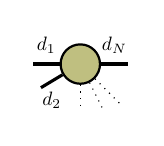
\begin{tikzpicture}[baseline=-0.5ex]
    \tikzset{tensor/.style = {minimum size = 0.5cm,shape = circle,thick,draw=black,inner sep = 0pt}, edge/.style = {thick,line width=.4mm},every loop/.style={}}
    \def\x{6}
    \node[tensor,fill=green!50!red!50!white] (T) at (\x,0) {$\At$};
    \draw[edge] (T) -- (\x-0.6,0)  node [midway,above] {\scalebox{0.7}{\dimcolor{$d_1$}}};
    \draw[edge] (T) -- (\x+0.6,0) node [midway,above] {\scalebox{0.7}{\dimcolor{$d_N$}}};
    \draw[edge] (T) -- (\x-0.5,-0.3) node [midway,below] {\scalebox{0.7}{\dimcolor{$d_2$}}};
    \draw[dotted] (T) -- (\x,-0.6);
    \draw[dotted] (T) -- (\x,-0.6);
    \draw[dotted] (T) -- (\x+0.5,-0.5);
    \draw[dotted] (T) -- (\x+0.3,-0.6);
    \end{tikzpicture}\in \RR^{d_1\times \cdots \times d_N} $\\
    三阶张量 $\At $ & $  
    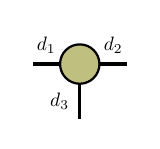
\begin{tikzpicture}[baseline=-0.5ex]
    \tikzset{tensor/.style = {minimum size = 0.5cm,shape = circle,thick,draw=black,inner sep = 0pt}, edge/.style = {thick,line width=.4mm},every loop/.style={}}
    \def\y{0}
    \def\x{0}
    \node[tensor,fill=green!50!red!50!white] (A) at (\x,\y){\scalebox{0.85}{$\At$}};
    \draw[edge] (\x+0.25,\y) -- (\x+0.6,\y)  node [midway,above] {\scalebox{0.7}{\dimcolor{$d_2$}}};
    \draw[edge] (\x-0.25,\y) -- (\x-0.6,\y)  node [midway,above] {\scalebox{0.7}{\dimcolor{$d_1$}}};
    \draw[edge] (\x,\y-0.25) -- (\x,\y-0.7)  node [midway,left] {\scalebox{0.7}{\dimcolor{$d_3$}}};
    \end{tikzpicture}\in \RR^{d_1 \times d_2 \times d_3}$\\
    张量元素 $\At_{i_1,i_2,i_3}$ &
    $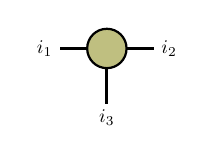
\begin{tikzpicture}[baseline=-0.5ex]
    \tikzset{tensor/.style = {minimum size = 0.5cm,shape = circle,thick,draw=black,inner sep = 0pt}, edge/.style = {thick,line width=.4mm},every loop/.style={}}
    \def\y{0}
    \def\x{0}
    \node[tensor,fill=green!50!red!50!white] (A) at (\x,\y){\scalebox{0.85}{$\At$}};
    \draw[edge] (\x+0.25,\y) -- (\x+0.6,\y)  node [very near end, right] {\scalebox{0.7}{\indcolor{$i_2$}}};
    \draw[edge] (\x-0.25,\y) -- (\x-0.6,\y)  node [very near end, left] {\scalebox{0.7}{\indcolor{$i_1$}}};
    \draw[edge] (\x,\y-0.25) -- (\x,\y-0.7)  node [very near end, below] {\scalebox{0.7}{\indcolor{$i_3$}}};
    \end{tikzpicture}\in \RR$ \\
    $\At\in\RR^{d_1\times d_2 \times d_3}$ 的模 2 矩阵化 & $ \Ab_{(2)}=\begin{tikzpicture}[baseline=\baseline]
    \tikzset{tensor/.style = {minimum size = 0.5cm,shape = circle,thick,draw=black,inner sep = 0pt}, edge/.style = {thick,line width=.4mm},every loop/.style={}}
    \def\y{0}
    \def\x{0}
    \node[tensor,fill=green!50!red!50!white] (A) at (\x,\y){\scalebox{0.85}{$\At$}};
    \draw[edge] (\x+0.2,\y+0.15) -- (\x+0.5,\y+0.15)-- (\x+0.5,\y+0.05) -- (\x+1,\y+0.05) node [midway,above]
    {\scalebox{0.7}{\dimcolor{$d_1$}}};
    \draw[edge] (\x+0.2,\y-0.15) -- (\x+0.5,\y-0.15)-- (\x+0.5,\y-0.05)-- (\x+1,\y-0.05) node [midway,below]
    {\scalebox{0.7}{\dimcolor{$d_3$}}};
    \draw[edge] (A) -- (\x-0.7,\y)node [midway,above]
    {\scalebox{0.7}{\dimcolor{$d_2$}}};
    \end{tikzpicture} \in \RR^{d_2\times d_1d_3}$ \\ $\At\in\RR^{d_1\times d_2\times d_3}$ 的向量化 & $\vectorize(\At)=
    \begin{tikzpicture}[baseline=\baseline]
    \tikzset{tensor/.style = {minimum size = 0.5cm,shape = circle,thick,draw=black,inner sep = 0pt}, edge/.style = {thick,line width=.4mm},every loop/.style={}}
    \def\y{0}
    \def\x{0}
    \node[tensor,fill=green!50!red!50!white] (A) at (\x,\y){\scalebox{0.85}{$\At$}};
    \draw[edge] (\x+0.15,\y+0.2) -- (\x+0.5,\y+0.2) -- (\x+0.5,\y+0.1) -- (\x+1,\y+0.1) node [midway,above]
    {\scalebox{0.7}{\dimcolor{$d_1$}}};
     \draw[edge] (A) -- (\x+1,\y)node [right]
    {\scalebox{0.7}{\dimcolor{$d_2$}}};

    \draw[edge] (\x+0.15,\y-0.2) -- (\x+0.5,\y-0.2)-- (\x+0.5,\y-0.1)-- (\x+1,\y-0.1) node [midway,below]
    {\scalebox{0.7}{\dimcolor{$d_3$}}};
    \end{tikzpicture}\in\RR^{d_1d_2d_3}$\\
    两个张量的外积 & $ \At \outprod \Bb =  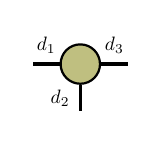
\begin{tikzpicture}[baseline=-0.5ex]
    \tikzset{tensor/.style = {minimum size = 0.5cm,shape = circle,thick,draw=black,inner sep = 0pt}, edge/.style = {thick,line width=.4mm},every loop/.style={}}
    \def\x{6}
    \def\y{0}
    \node[tensor,fill=green!50!red!50!white] (A) at (\x,\y) {$\At$};
    \draw[edge] (A) -- (\x-0.6,\y) node [midway,above] {\scalebox{0.7}{\dimcolor{$d_1$}}};
    \draw[edge] (A) -- (\x+0.6,\y) node [midway,above] {\scalebox{0.7}{\dimcolor{$d_3$}}};
    \draw[edge] (A) -- (\x,\y-0.6) node [midway,left] {\scalebox{0.7}{\dimcolor{$d_2$}}};
    \end{tikzpicture}
    \hspace{0.3cm}
    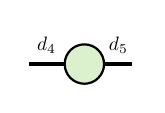
\begin{tikzpicture}[baseline=-0.5ex]
    \tikzset{tensor/.style = {minimum size = 0.5cm,shape = circle,thick,draw=black,inner sep = 0pt}, edge/.style = {thick,line width=.4mm},every loop/.style={}}
    \def\x{6}
    \def\y{0}
    \node[tensor,fill=green!70!red!20!white] (B) at (\x+1,\y) {$\Bb$};
    \draw[edge] (B) -- (\x+0.3,0) node [midway,above] {\scalebox{0.7}{\dimcolor{$d_4$}}};
    \draw[edge] (B) -- (\x+1.6,0)node [midway,above] {\scalebox{0.7}{\dimcolor{$d_5$}}};
    \end{tikzpicture} \in \RR^{d_1\times d_2 \times d_3 \times d_4\times d_5}$ \\
    \\
    两个张量的内积 &$\inner{\At}{\Bt} = \begin{tikzpicture}[baseline=\baseline]
    \tikzset{tensor/.style = {minimum size = 0.5cm,shape = circle,thick,draw=black,inner sep = 0pt}, edge/.style = {thick,line width=.4mm},every loop/.style={}}
    \def\y{0}
    \def\x{0}
    \node[tensor,fill=green!50!red!50!white] (St) at (\x,\y){\scalebox{0.85}{$\At$}};
    \node[tensor,fill=green!50!red!50!white] (Tt) at (\x+1,\y){\scalebox{0.85}{$\Bt$}};
    \draw[edge] (St) -- (Tt);
    \draw[edge] (St) to [out=45,in=135] (Tt);
    \draw[edge] (St) to [out=-45,in=-135] (Tt);
    \node[draw=none] () at (\x+0.5,\y+0.5) {\scalebox{0.7}{\dimcolor{$d_1$}}};
    \node[draw=none] () at (\x+0.5,\y+0.15) {\scalebox{0.7}{\dimcolor{$d_2$}}};
    \node[draw=none] () at (\x+0.5,\y-0.5) {\scalebox{0.7}{\dimcolor{$d_3$}}};
\end{tikzpicture} \in\RR $\\
    \\
    张量的 Frobenius 范数 & $\norm{\At}_F^2 = \begin{tikzpicture}[baseline=\baseline]
    \tikzset{tensor/.style = {minimum size = 0.5cm,shape = circle,thick,draw=black,inner sep = 0pt}, edge/.style = {thick,line width=.4mm},every loop/.style={}}
    \def\y{0}
    \def\x{0}
    \node[tensor,fill=green!50!red!50!white] (St) at (\x,\y){\scalebox{0.85}{$\At$}};
    \node[tensor,fill=green!50!red!50!white] (Tt) at (\x+1,\y){\scalebox{0.85}{$\At$}};
    \draw[edge] (St) -- (Tt);
    \draw[edge] (St) to [out=45,in=135] (Tt);
    \draw[edge] (St) to [out=-45,in=-135] (Tt);
    \node[draw=none] () at (\x+0.5,\y+0.5) {\scalebox{0.7}{\dimcolor{$d_1$}}};
    \node[draw=none] () at (\x+0.5,\y+0.15) {\scalebox{0.7}{\dimcolor{$d_2$}}};
    \node[draw=none] () at (\x+0.5,\y-0.5) {\scalebox{0.7}{\dimcolor{$d_3$}}};
\end{tikzpicture}\in\RR$\\
    \\
    两个张量的 Kronecker 积 & $\At\kron\Bt=   \begin{tikzpicture}[baseline=-0.5ex]
    \tikzset{tensor/.style = {minimum width = 2.2cm,minimum height = 0.5cm,shape = rounded rectangle,thick,draw=black,inner sep = 0pt}, edge/.style = {thick,line width=.4mm},every loop/.style={}}
    \def\x{0.5}
    \def\y{0.25}
    \draw[edge] (\x-0.85,\y-0.3) -- (\x-0.85,\y-0.6) -- (\x-0.65,\y-0.6) -- (\x-0.65,\y-0.8);
    \draw[edge] (\x-0.35,\y-0.3) -- (\x-0.35,\y-0.6) -- (\x-0.55,\y-0.6) -- (\x-0.55,\y-0.8)node[below]{\scalebox{0.7}{\dimcolor{$d_1d_4$}}};
    \draw[edge] (\x+0.85,\y-0.3) -- (\x+0.85,\y-0.6) -- (\x+0.65,\y-0.6) -- (\x+0.65,\y-0.8);
    \draw[edge] (\x+0.35,\y-0.3) -- (\x+0.35,\y-0.6) -- (\x+0.55,\y-0.6) -- (\x+0.55,\y-0.8)node[below]{\scalebox{0.7}{\dimcolor{$d_3d_6$}}};
    \draw[edge](\x-0.25,\y-0.3)--(\x-0.25,\y-0.6)-- (\x-0.05,\y-0.6)--(\x-0.05,\y-0.8);
    \draw[edge](\x+0.25,\y-0.3)--(\x+0.25,\y-0.6)-- (\x+0.05,\y-0.6)--(\x+0.05,\y-0.8)node[below]{\scalebox{0.7}{\dimcolor{$d_2d_5$}}};
    \node[tensor,fill=green!30!white] (At) at (\x,\y-0.2){$\At\kron\Bt$};
    \end{tikzpicture}\in\RR^{d_1d_4\times d_2d_5\times d_3d_6}$\\

    二阶张量~（矩阵）$\Ab$ & $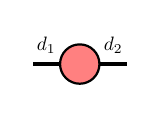
\begin{tikzpicture}[baseline=-0.5ex]
    \tikzset{tensor/.style = {minimum size = 0.5cm,shape = circle,thick,draw=black,inner sep = 0pt}, edge/.style = {thick,line width=.4mm},every loop/.style={}}
    \def\x{0}
    \def\y{0}
    \node[tensor,fill=red!50!white] (A) at (\x+1,\y){\scalebox{0.85}{$\Ab$}};
    \draw[edge] (\x+1.25,\y) -- (\x+1.6,\y)  node [midway,above] {\scalebox{0.7}{\dimcolor{$d_2$}}};
    \draw[edge] (\x+0.75,\y) -- (\x+0.4,\y)  node [midway,above] {\scalebox{0.7}{\dimcolor{$d_1$}}};
    \end{tikzpicture}\in\RR^{d_1\times d_2}$\\
    \\
    单位矩阵 &$\Ib_d =  \begin{tikzpicture}[baseline=\baseline]
    \tikzset{tensor/.style = {minimum size = 0.5cm,shape = circle,thick,draw=black,inner sep = 0pt}, edge/.style   = {thick,line width=.4mm},every loop/.style={}}
    \def\y{0}
    \def\x{0}
    \draw[edge](\x,\y)--(\x+1.5,\y);
    \node[draw=none] () at (\x+0.75,\y+0.15) {\scalebox{0.7}{\dimcolor{$d$}}};
    \end{tikzpicture}\in\RR^{d\times d}$\\  
    \\
    Kronecker delta 记号 &     $\begin{tikzpicture}[baseline=\baseline]
    \tikzset{tensor/.style = {minimum size = 0.5cm,shape = circle,thick,draw=black,inner sep = 0pt}, edge/.style   = {thick,line width=.4mm},every loop/.style={}}
    \def\y{0}
    \def\x{0}
    \draw  node[fill = black,circle,inner sep=0pt,minimum size=4pt] (m) at (\x,\y) {};
    \draw  node[fill = black,circle,inner sep=0pt,minimum size=4pt] (m) at (\x,\y) {};
    \draw[edge] (m) -- (\x-0.6,0) node [very near end,left] {\scalebox{0.7}{\indcolor{$i$}}};
    \draw[edge] (m) -- (\x+0.6,0) node [very near end,right]
    {\scalebox{0.7}{\indcolor{$j$}}};
    \node[draw=none] at (\x+1,\y) {\scalebox{1}{\textcolor{black}{$=$}}};;
    \draw[edge] (\x+1.3,\y) -- (\x+2.5,\y) node [very near start,left=0.05cm] {\scalebox{0.7}{\indcolor{$i$}}} node [very near end,right=0.05cm] {\scalebox{0.7}{\indcolor{$j$}}};
    \end{tikzpicture} = \delta_{ij} = \begin{cases}
      1 & \text{if } i=j\\
      0 & \text{otherwise},
    \end{cases}
    =
    \Ib_{ij}$\\
    
    Khatri-Rao 积  &  
    $\Ab\krao\Bb=  \begin{tikzpicture}[baseline=\baseline]
    \tikzset{tensor/.style = {minimum size = 0.5cm,shape = circle,thick,draw=black,inner sep = 0pt}, edge/.style   = {thick,line width=.4mm},every loop/.style={}}
    \def\y{0}
    \def\x{0}
    \node[tensor,fill=red!50!white] (A) at (\x,\y){$\Ab$};
    \node[tensor,fill=blue!50!white] (B) at (\x+1,\y){$\Bb$};
    \draw[edge] (\x,\y+0.25) -- (\x,\y+0.5) -- (\x+0.5,\y+0.7);
    \draw[edge] (\x+1,\y+0.25) -- (\x+1,\y+0.5) -- (\x+0.5,\y+0.7);
    \draw[edge] (\x+0.5,\y+0.7) -- (\x+0.5,\y+1.2)node [midway,right] {\scalebox{0.7}{\dimcolor{$R$}}};
    \draw  node[fill = black,circle,inner sep=0pt,minimum size=4pt] (m) at (\x+0.5,\y+0.7) {};
    \draw[edge] (\x,\y-0.25) -- (\x,\y-0.7);
    \draw[edge] (\x+1,\y-0.25) -- (\x+1,\y-0.7);
    \draw[edge] (\x+1,\y-0.7) -- (\x+0.5,\y-0.7) -- (\x+0.5,\y-1)node [below] {\scalebox{0.7}{\dimcolor{$d_1d_2$}}};
    \draw[edge] (\x+1,\y-0.25) -- (\x+1,\y-0.7);
    \draw[edge] (\x,\y-0.7) -- (\x+0.4,\y-0.7) -- (\x+0.4,\y-1);
    \end{tikzpicture}\in\RR^{d_1d_2\times R}$\\
    Hadamard 积 & $\Ab\hadam\Bb =  \begin{tikzpicture}[baseline=\baseline]
    \tikzset{tensor/.style = {minimum size = 0.5cm,shape = circle,thick,draw=black,inner sep = 0pt}, edge/.style   = {thick,line width=.4mm},every loop/.style={}}
    \def\y{0}
    \def\x{0}
    \node[tensor,fill=red!50!white] (A) at (\x,\y){$\Ab$};
    \node[tensor,fill=blue!50!white] (B) at (\x+1,\y){$\Bb$};
    \draw[edge] (\x,\y+0.25) -- (\x,\y+0.5) -- (\x+0.5,\y+0.7);
    \draw[edge] (\x+1,\y+0.25) -- (\x+1,\y+0.5) -- (\x+0.5,\y+0.7);
    \draw[edge] (\x+0.5,\y+0.7) -- (\x+0.5,\y+1)node [midway,right] {\scalebox{0.7}{\dimcolor{$d_1$}}};
    \draw  node[fill = black,circle,inner sep=0pt,minimum size=4pt] (m) at (\x+0.5,\y+0.7) {};
    \draw[edge] (\x,\y-0.25) -- (\x,\y-0.5) -- (\x+0.5,\y-0.7);
    \draw[edge] (\x+1,\y-0.25) -- (\x+1,\y-0.5) -- (\x+0.5,\y-0.7);
    \draw[edge] (\x+0.5,\y-0.7) -- (\x+0.5,\y-1)node [midway,right] {\scalebox{0.7}{\dimcolor{$d_2$}}};
    \draw  node[fill = black,circle,inner sep=0pt,minimum size=4pt] (m) at (\x+0.5,\y-0.7) {};
    \end{tikzpicture}\in\RR^{d_1\times d_2}$ \\ 
    一阶张量~（向量）$\ab$
    &     $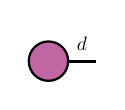
\begin{tikzpicture}[baseline=-0.5ex]
    \tikzset{tensor/.style = {minimum size = 0.5cm,shape = circle,thick,draw=black,inner sep = 0pt}, edge/.style = {thick,line width=.4mm},every loop/.style={}}
    \def\y{0}
    \def\x{0}
    \node[tensor,fill=blue!40!red!60!white] (a) at (\x,\y){\scalebox{0.85}{$\ab$}};
    \draw[edge] (\x+0.25,\y) -- (\x+0.6,\y)  node [midway,above] {\scalebox{0.7}{\dimcolor{$d$}}};
\end{tikzpicture}\in\RR^d$\\
\\
    零阶张量~（标量）$a$ &
    $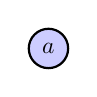
\begin{tikzpicture}[baseline=-0.5ex]
    \tikzset{tensor/.style = {minimum size = 0.5cm,shape = circle,thick,draw=black,inner sep = 0pt}, edge/.style = {thick,line width=.4mm},every loop/.style={}}
    \def\y{0}
    \def\x{0}
    \node[tensor,fill=blue!20!white] (a) at (\x,\y){\scalebox{0.85}{$a$}};
    \end{tikzpicture}\in\RR$
    
    \end{tabular}
 \end{table}
